\documentclass[9pt]{beamer}

\usepackage[utf8]{inputenc}
\usepackage{eurosym}
\RequirePackage[francais]{babel}
%\usepackage{url}
%\usepackage{etex}
%\usepackage{enumitem}
%\usepackage{multicol}
\usepackage{xcolor}
%\usepackage{bbm}
%\usepackage{amsmath,amsthm,amssymb}
%\usepackage[official]{eurosym}
%\usepackage{pifont}
%\usepackage{exercise}
%\usepackage{graphics}
%\usepackage{array,multirow,makecell}
\usepackage{verbatim}
%\usepackage[dvipsnames]{pstricks}
\usepackage{pstricks-add,pst-plot,pst-text,pst-tree,pst-eps,pst-fill,pst-node,pst-math,pst-blur,pst-func}
%\usepackage{pgf,tikz}
%\usepackage{tipfr}
%\usepackage{thmbox}
%\usepackage{calc}
%\usepackage{ifthen}
%\usepackage{pdfpages}
%\usepackage{colortbl}
%\usepackage{sagetex}
%\usetikzlibrary{arrows,patterns}
%\input tabvar
%\usepackage{tkz-tab}
%\usepackage{listings}
%\usepackage[np]{numprint}
%\usepackage{fancybox,fancyhdr}
%\usepackage{thmtools}
%\usepackage{bclogo}
%\usepackage{lastpage}

\usepackage{tabularx}
\usepackage{array,multirow,makecell}
\usetheme{Madrid}
%\usetheme{Bergen}
\usecolortheme{beaver}
 
%Information to be included in the title page:
\title{Algorithmique}
\subtitle{Parcours et tri d'un tableau}
\author{Yannick CHISTEL}
\institute{Lycée Dumont d'Urville - CAEN}
\date{Mars 2020}
 
%----------------------------------------------------------------------------------------------- 
% 							Commandes Tableaux
%-----------------------------------------------------------------------------------------------
\setcellgapes{1pt}
\makegapedcells
\newcolumntype{R}[1]{>{\raggedleft\arraybackslash }b{#1}}
\newcolumntype{L}[1]{>{\raggedright\arraybackslash }b{#1}}
\newcolumntype{C}[1]{>{\centering\arraybackslash }b{#1}}

\definecolor{vert}{rgb}{0,0,1}

\newcommand{\esp}{\hspace{0.5cm}}
\newcommand{\espp}{\hspace{1cm}}
\newcommand{\esppp}{\hspace{1.5cm}}

\newcounter{num}
\setcounter{num}{0}
 
\begin{document}
 
\frame{\titlepage}

\begin{frame}
\frametitle{Algorithme}

\begin{block}{Définition}
Un \textbf{algorithme} est l'écriture en langage naturel d'une suite d'instructions répondant à une problématique donnée.

Un algorithme peut être traduit dans n'importe quel langage de programmation tout en respectant la structure globale de celui-ci.

Des mots clés seront utilisés comme : 
\begin{itemize}
\item \textbf{si}, \textbf{alors} et \textbf{sinon} pour traiter les structures conditionnelles;
\item \textbf{Pour} et \textbf{Tant que} pour traiter les structures itératives;
\item L'\textbf{affectation} d'une valeur à une variable se note par la flèche $\longleftarrow$
\end{itemize}
\end{block}

\begin{exampleblock}{Exemple}
Voici un algorithme de recherche de la valeur minimale dans un tableau T :\medskip

$m \longleftarrow T[0]$\\
Pour $i$ allant de 1 à longueur(T):\\
\esp Si $T[i]<m$ alors $m=T[i]$\\
Fin pour
\end{exampleblock}

\end{frame}


\begin{frame}
\frametitle{Algorithme de tri}

\begin{block}{Introduction}
Il est souvent plus simple de traiter des données lorsque celles-ci sont triées. Il existe deux algorithmes pour trier des valeurs : le \textbf{tri par sélection} et le \textbf{tri par insertion}.
\end{block}

\begin{block}{Principe du tri par sélection}
On sépare en 2 parties les données à trier. La première partie contient les données déjà triées et la seconde contient les données non triées.\smallskip

On cherche la plus petite valeur dans la seconde partie et on la place au début de celle-ci. Elle devient alors la plus grande valeur de la première partie triée.\smallskip

On recommence jusqu'à avoir la seconde partie vide.
\end{block}

\begin{block}{Principe du tri par insertion}
On sépare en 2 parties les données à trier. La première partie contient les données déjà triées et la seconde contient les données non triées.\smallskip

On prend la première valeur de la partie non triée (la plus à gauche) et on l'insère dans la partie triée en décalant d'un rang vers la droite toutes les valeurs qui lui sont supérieures.\smallskip

On recommence jusqu'à avoir la seconde partie vide.
\end{block}

\end{frame}

\begin{frame}
\frametitle{Algorithme de tri par sélection}

\begin{block}{Algorithme}
Voici une écriture de l'algorithme de tri par sélection:\medskip

$i \longleftarrow 1$\\
tant que $i < \text{longueur(t)}$:   //boucle 1\\
\esp $j \longleftarrow i$\\
\esp $\text{min} \longleftarrow i$\\
\esp tant que $j <= \text{longueur(t)}$:   //boucle 2\\
\espp si $t[j] < t[min]$:\\
\esppp $\text{min} \longleftarrow j$\\
\espp fin si\\
\esp $j \longleftarrow j+1$\\
\esp fin tant que\\
\esp si $min \neq i$ :\\
\espp échanger t[i] et t[min]\\
\esp fin si\\
\esp $i \longleftarrow i+1$\\
fin tant que
\end{block}

\end{frame}


\begin{frame}
\frametitle{Algorithme de tri par sélection}

\begin{exampleblock}{Exemple}
\begin{minipage}{8.4cm}
Soit le tableau de valeurs $T=[15,11,19,8]$
\begin{enumerate}
\item $i=1$ : on cherche la valeur minimale du tableau, entre $j=1$ et $j=4$ : ici c'est 8 pour $j=4$. On mémorise l'indice dans la variable $\text{min}=4$.\\
$i \neq \text{min}$, on échange les 2 valeurs: $8 \longleftrightarrow 15$
\item $i=2$, on cherche la valeur minimale du tableau, entre $j=2$ et $j=4$ : ici c'est pour $j=2$. On mémorise l'indice dans la variable $\text{min}=2$.\\
$i = \text{min} = 4$, on n'échange pas les valeurs.
\item $i=3$, on cherche la valeur minimale du tableau, entre $j=3$ et $j=4$ : ici c'est pour $j=4$. On mémorise l'indice dans la variable $\text{min}=4$.\\
$i \neq \text{min}$, on échange les 2 valeurs : $19 \longleftrightarrow 15$
\item $i=4$, on cherche la valeur minimale du tableau, entre $j=4$ et $j=4$ donc pour $j=4$. On mémorise l'indice dans la variable $\text{min}=4$.\\
$i = \text{min} = 4$, on n'échange pas les valeurs.
\end{enumerate}
\end{minipage}\hfill
\begin{minipage}{3.4cm}
\includegraphics[scale=0.5]{img/algo-tri-select.eps}
\end{minipage}
\end{exampleblock}
\end{frame}

\begin{frame}
\frametitle{Algorithme de tri par insertion}

\begin{block}{Algorithme}
Voici une écriture de l'algorithme de tri par insertion:\medskip
$j \longleftarrow 2$\\
tant que $j <= \text{longueur}(t)$:   //boucle 1\\
\esp $i \longleftarrow j-1$\\
\esp $k \longleftarrow t[j]$\\
\esp tant que $i>0$ et que $t[i]>k$:   //boucle 2\\
\espp $t[i+1] \longleftarrow t[i]$\\
\espp $i \longleftarrow i-1$\\
\esp fin tant que\\
\esp $t[i+1] \longleftarrow k$\\
\esp $j \longleftarrow j+1$\\
fin tant que
\end{block}

\end{frame}

\begin{frame}
\frametitle{Algorithme de tri par insertion}

\begin{exampleblock}{Exemple}
\begin{minipage}{8.4cm}
Soit le tableau de valeurs $T=[15,11,19,8]$
\begin{enumerate}
\item $j=2$, $k=T[2]=11$ et $i=1$ : on compare la valeur $11$ avec la valeur $15$. Comme elle est inférieure on décale à droite la valeur $15$ en $j=2$ et on insère la valeur $11$ en $i=1$.
\item $j=3$, $k=T[3]=19$ et $i=2$ : on compare la valeur $19$ avec la valeur $15$. Comme elle est supérieure on sort de la boucle ($T[2]>k]$), on garde $T[3]=19$ et on passe à $j=4$.
\item $j=4$, $k=T[4]=8$ et $i=3$:
\begin{itemize}
\item on compare la valeur $8$ avec la valeur $19$. Comme elle est inférieure on décale à droite la valeur $19$ en $i=4$ et $i$ passe à $2$;
\item on compare la valeur $8$ avec la valeur $15$. Comme elle est inférieure on décale à droite la valeur $15$ en $i=3$ et $i$ passe à $1$;
\item on compare la valeur $8$ avec la valeur $11$. Comme elle est inférieure on décale à droite la valeur $11$ en $i=2$ et $i$ passe à $0$. On sort de la boucle et $T[1]=8$.
\end{itemize}
\end{enumerate}
\end{minipage}\hfill
\begin{minipage}{3.4cm}
\includegraphics[scale=0.5]{img/algo-tri-inser.eps}
\end{minipage}
\end{exampleblock}
\end{frame}

\begin{frame}
\frametitle{Le tri de tableaux en python}

\begin{block}{Introduction}
Les langages de programmation possèdent souvent leurs propres fonctions de tri.

En python, il existe pour les tableaux, 2 fonctions de tri qui sont \textbf{sort()} et \textbf{sorted()}
\begin{enumerate}
\item La fonction \textbf{sort()} s'applique sur un tableau et trie ses valeurs par ordre croissant. 

Le tableau initial est modifié.
\begin{center}
\includegraphics[scale=0.5]{img/algotri1.eps}
\end{center}
\item La fonction \textbf{sorted()} prend en argument un tableau et crée un nouveau tableau avec les valeurs du tableau initial triées dans l'ordre croissant. 

Le tableau initial n'est pas modifié.
\begin{center}
\includegraphics[scale=0.5]{img/algotri2.eps}
\end{center}
\end{enumerate}
\end{block}

\end{frame}

\begin{frame}
\frametitle{Recherche dichotomique}

\begin{block}{Principe}
La \textbf{dichotomie} est un mot d'origine greque qui signifie \og diviser en deux \fg.

La recherche d'une valeur dans un tableau peut être facilitée si celui-ci est trié. Dans ce cas, on divise successivement le tableau en 2 jusqu'à atteindre la valeur cherchée.
\end{block}

\begin{exampleblock}{Exemple}
\begin{minipage}{7cm}
Soit $T=[5,9,12,14,15,16,19,20,23,25]$
\begin{enumerate}
\item On cherche le nombre $12$. Il est inférieur à la plus grande valeur du tableau.
\item On calcule la valeur de l'indice situé au milieu du tableau: $m=4$. \smallskip

On compare la valeur $T[4]$ avec $12$:
\begin{itemize}
\item si $12 < T[4]$ alors 12 est dans la première moitié du tableau;
\item si $12 > T[4]$ alors 12 est dans la seconde moitié du tableau;
\item si $12=T[4]$ alors le nombre est trouvé
\end{itemize}
\item On répète ce processus jusqu'à avoir un tableau réduit à une valeur ou vide !
\end{enumerate}
\end{minipage}
\begin{minipage}{5cm}
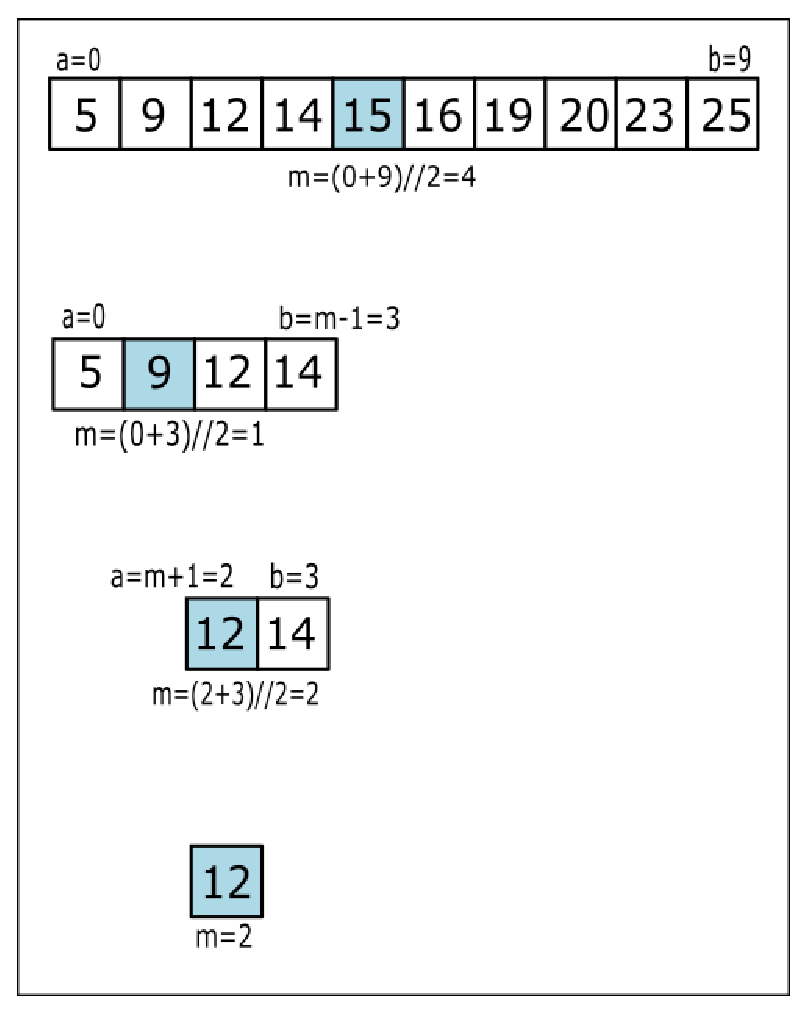
\includegraphics[scale=0.35]{img/dichotomie.eps}
\end{minipage}

\end{exampleblock}
\end{frame}

\begin{frame}
\frametitle{Recherche dichotomique}

\begin{block}{Algorithme}
Voici une écriture de l'algorithme de recherche dichotomique dans un \textbf{tableau trié} :\medskip

$t$ désigne un tableau trié\\
$v$ est la valeur cherchée dans le tableau\\
$a$, $b$ et $m$ sont les indices de position des valeurs dans le tableau.\medskip

$a \longleftarrow 1$ \hfill ...\textit{première valeur du tableau}\\
$b \longleftarrow \text{longueur}(t)$  \hfill ...\textit{dernière valeur du tableau}\\
\textbf{tant que} $a <= b$: \\
\esp $m \longleftarrow (a+b)//2 $ \hfill ...\textit{m est la position au milieu} \\
\esp \textbf{si} $v<t[m]$ alors $b=m-1$ \hfill ...\textit{v se trouve dans la première moitié}\\
\esp \textbf{sinon si} $v>t[m]$ alors $a=m+1$  \hfill ...\textit{v se trouve dans la seconde moitié}\\
\esp \textbf{sinon} la valeur est trouvée en $m$\\
fin tant que\\
La valeur n'est pas trouvée
\end{block}

\end{frame}


\begin{frame}
\frametitle{Terminaison de l'algorithme}

\begin{block}{Variant de boucle}
On appelle \textbf{variant de boucle} une quantité entière qui:
\begin{itemize}
\item doit être positive ou nulle pour rester dans la boucle;
\item décroit strictement à chaque itération
\end{itemize}
Si on trouve une telle quantité dans une boucle while, celle-ci se termine.
\end{block}

\begin{block}{Preuve de la terminaison}
Dans l'algorithme de recherche par dichotomie, le variant de boucle est $b-a$.
\begin{itemize}
\item Ce nombre est clairement supérieur ou égal à 0 puisque $a<=b$.
\item Vérifions qu'elle décroît en distinguant 3 cas :
\begin{enumerate}
\item[cas 1:] $t[m]==v$ alors on sort de la boucle. \medskip
\item[cas 2:] \begin{minipage}{6cm}
$t[m]>v$ donc $b'-a < m-a < b-a$ donc la quantité $b-a$ décroit.
\end{minipage}\hfill
\begin{minipage}{3.5cm}
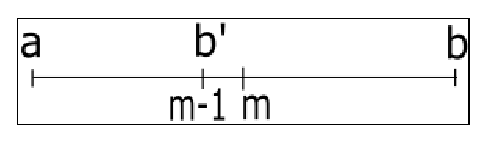
\includegraphics[scale=0.4]{img/cas2.eps}
\end{minipage}\medskip
\item[cas 3:] \begin{minipage}{6cm}
$t[m]<v$ donc $b-a' < b-m < b-a$ donc la quantité $b-a$ décroit.
\end{minipage}\hfill
\begin{minipage}{3.5cm}
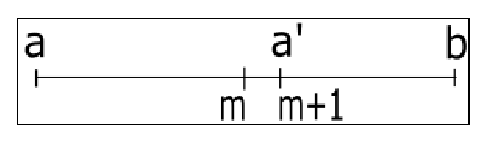
\includegraphics[scale=0.4]{img/cas3.eps}
\end{minipage}
\end{enumerate}
\end{itemize}
$b-a$ est un variant de boucle positif qui décroit, assurant la terminaison de la \textbf{boucle while}.
\end{block}
\end{frame}


\begin{frame}
\frametitle{Coût, efficacité, complexité d'un algorithme}

\begin{block}{Introduction}
Déterminer l'efficacité d'un algorithme est important. Certaines instructions sons répétées de nombreuses fois et peuvent finir par prendre beaucoup de temps. On cherche alors à calculer un ordre de grandeur du nombre de calculs réalisés.
\begin{enumerate}
\item La recherche d'une valeur dans un tableau (minimum, maximum) est de complexité \textbf{linéaire}. Le nombre de calculs (comparaisons) est proportionnel à la dimension $n$ du tableau. On note cette complexité par $O(n)$.
\item Le tri d'un tableau par sélection ou insertion est de complexité \textbf{quadratique}. Le nombre d'opérations est proportionnel au carré de la dimension $n$ du tableau. On note cette complexité par $O(n^2)$.
\item La recherche par dichotomie est de complexité logarithmique. On la note $O(\log_{2}(n))$.
\end{enumerate}
\end{block}

\begin{block}{Propriété}
On peut comparer l'efficacité des algorithmes en comparant leur complexité. Pour un tableau de dimension $n$, on a : $$O(\log_{2}(n)) < O(n) < O(n^2)$$
\end{block}

\end{frame}
\end{document}

